\section{对数 GLSM（Qile Chen）}%
\label{sec:Log GLSM (Qile Chen)}

设 \(X\) 为光滑射影簇（甚至可以是 DM 栈）。设 \(E\) 为 \(X\) 上的一个向量丛，带有截面 \(s \in H^0(E)\)，它定义了一个具有期望余维数的光滑零截面 \(Z\)。我们称 \(X\) 与 \(E\) 为外围（ambient），称 \(s\) 与 \(Z\) 为完全交。

\begin{quest}
    \(Z\) 的 GW 理论与 \((X, E)\) 的 GW 理论之间有什么关系？
\end{quest}

当 \(g = 0\) 时，Givental 与 Lian-Liu-Yau 利用这一关系计算了完全交的 GW 不变量；当 \(g = 1\) 时，这一工作由 Zinger 完成。一般地，有两种途径：(N)MSP 与对数 GLSM。在本系列讲座中，我们将讨论对数 GLSM。\footnote{Qile 让对 MSP 有疑问的听众去询问本笔记的作者与 Yang Zhou。}

\subsection{R-映射}%
\label{sub:R-maps}

我们将考虑 \textit{R-环面} \(\C^{\times}_{\omega} \coloneqq \C^{\times}\)。它有一个权重 \(1\) 的表示，我们称之为 \(\C_{\omega}\)。它下降为 \(B \C_{\omega}^{\times}\) 上的线丛 \(\mc{L}_{\omega} \coloneqq [\C_{\omega} / \C^{\times}_{\omega}]\)。R-映射的目标是栈
\[ \P \to B \C^{\times}_{\omega} \]
它们是 DM 型的、分离的且（对数）光滑的。现在，一个 R-映射由一个（2-）交换图组成
\begin{equation*}
\begin{tikzcd}
    & \mf{P} \ar{d} \\
    C \ar{ur}{f} \ar{r}[swap]{\omega^{\log}} \ar{d} & B \C_{\omega}^{\times} \\
    S.
\end{tikzcd}
\end{equation*}
这里，曲线可以是预稳定的、扭曲的、对数的，甚至是穿孔的。

\begin{exm}
    我们的第一个例子是稳定映射。令 \(\mf{P} = B\C_{\omega}^{\times}\)。因为在图
    \begin{equation*}
    \begin{tikzcd}
        & X \times B\C_{\omega}^{\times} \ar{d} \\
        C \ar{ur} \ar{r} & B \C_{\omega}^{\times}
    \end{tikzcd}
    \end{equation*}
    中，竖直箭头是第二投影，我们看到这归结为到 \(X\) 的一个映射。
\end{exm}

\begin{exm}
    考虑映射
    \begin{equation*}
    \begin{tikzcd}
        & \mc{L}_{\omega} \ar{d} \\
        C \ar{ur}{f} \ar{r} & B \C_{\omega}^{\times}.
    \end{tikzcd}
    \end{equation*}
    若假设 \(C\) 无标记，我们看到该映射的数据只不过是 \(\omega_C\) 的一个截面，因此我们恢复了全纯微分。
\end{exm}

\begin{exm}
    考虑由 \(z \mapsto z^{r_{\mr{in}}}\) 给出的态射 \(\C^{\times}_R \to \C^{\times}_{\omega}\)。于是我们看到
    \[ \mc{L}_R^{\otimes r_{\mr{in}}} \simeq \mc{L}_{\omega} |_{B \C_R^{\times}}. \]
    现在，图
    \begin{equation*}
    \begin{tikzcd}
        & B \C_R^{\times} \ar{d} \\
        C \ar{ur}{f} \ar{r} & B \C_{\omega}^{\times}
    \end{tikzcd}
    \end{equation*}
    在 \(C\) 无标记时等价于一个线丛 \(\mc{L}_R|_C\) 和一个同构 \(\mc{L}_R^{\otimes r_{\mr{in}}} \simeq \omega_C\) 的数据。或者，我们可以考虑形如
    \begin{equation*}
    \begin{tikzcd}
        & \mc{L}_R \ar{d} \\
        & B \C_R^{\times} \ar{d} \\
        C \ar{uur}{f} \ar{r} & B \C_{\omega}^{\times},
    \end{tikzcd}
    \end{equation*}
    的 R-映射，它们参数化了带有一个 R-旋线丛和一个截面的曲线。
\end{exm}

\begin{exm}
    设 \(X\) 为光滑射影簇。那么考虑形如
    \begin{equation*}
    \begin{tikzcd}
        & E^{\vee} \boxtimes \mc{L}_{\omega} \ar{d} \\
        & X \times B \C_{\omega}^{\times} \ar{d} \\
        C \ar{uur}{f} \ar{r} & B \C_{\omega}^{\times}.
    \end{tikzcd}
    \end{equation*}
    的 R-映射。这等价于一个映射 \(C \to X\) 连同截面 \(\rho \in H^0(E^{\vee}|_C \otimes \omega_C)\)。
\end{exm}

我们将考虑 GW 情形的目标。
考虑外围 \((X, E)\) 的数据。那么我们令 \(\mf{P}^{\circ} \coloneqq E^{\vee} \boxtimes \mc{L}_{\omega}\)。态射 \(\mf{P}^{\circ} \to B \C_{\omega}^{\times}\) 性质很好，但它不是本征的。为弥补这一点，我们考虑对数栈
\[ \mf{P} = ( \P(E^{\vee} \boxtimes \mc{L}_{\omega} \oplus \mc{O}) , \infty). \]
因为在光滑栈中有一个光滑除子，映射 \(\mf{P} \to B \C_{\omega}^{\times}\) 是本征且对数光滑的。注意到我们有零截面
\[ 0_{\mf{P}} \subset \mf{P}^{\circ} \subset \mf{P} \supset \infty. \]

我们现在考虑 r-旋情形的目标。考虑对数栈
\[ (\P(\mc{L}_R^{\oplus n} \oplus \mc{O}), \infty) = \mf{P} \to B \C_R^{\times} \to B \C_{\omega}^{\times}. \]
该态射是本征且对数光滑的。

\subsection{对数与穿孔 R-映射}%
\label{sub:Log and punctured R-maps}

我们考虑图
\begin{equation*}
\begin{tikzcd}
    & \mf{P} \ar{d} \\
    C \ar{ur}{f} \ar{r}[swap]{\omega^{\log}} \ar{d} & B \C_{\omega}^{\times} \\
    S
\end{tikzcd}
\end{equation*}
其中 \(C \to S\) 是一条对数或穿孔（可能扭曲）曲线，\(S\) 是一个 fs 对数概形。GW 情形的稳定性条件是 \(f\) 可表且
\[ (\omega_{\log})^{1+\delta} + H^{\otimes k} \otimes f^* \mc{O}(\infty) > 0 \]
对所有 \(0 < \delta \ll 1\) 与 \(k \gg 1\) 成立，其中 \(H\) 是 \(X\) 的粗模空间上的一个丰沛线丛。对于穿孔 R-映射，我们还要求预稳定性。

\begin{exm}
    考虑全纯微分的情形。考虑 \(f \in H^0(\omega_C)\)，使其所有零点都集中在单个 Weierstrass 点处，其中 \(C\) 的亏格为 \(2\)。若考虑 \(\lim_{\lambda \to \infty} \lambda \cdot f\)，则该极限由一个完全映到 \(\infty\) 的亏格 \(2\) 分支和一个记住了该零点的有理分支组成。
\end{exm}

我们现在讨论对数或穿孔 R-映射的热带化。回忆，一个图
\[ \ul{G} = (\V, \H, \imath \colon \H \to \H, v \colon \H \to \V) \]
由顶点集合 \(\V\)、半边集合 \(\H\)、半边上的一个对合 \(\imath\) 和一个从半边到顶点的根映射组成。那么我们令腿的集合 \(\L\) 为
\[ \L = \ab\{ h \in \H \mid \imath(h) = h\}. \]
边是由对合相互对应的不同半边所成的对：
\[ \E = \ab\{ \ab\{h, \hat{h}\} \mid \imath(h) = \hat{h} \neq h \}. \]
现在，带装饰的图是一个图连同亏格函数
\[ g \colon \V \to \N, \]
一个指定
\[ r \colon \H \to \N, \]
以及一个排序
\[ m \colon \L \to \ab\{0, \ldots, n\}. \]

\begin{exm}
    \leavevmode\par
    \begin{center}
    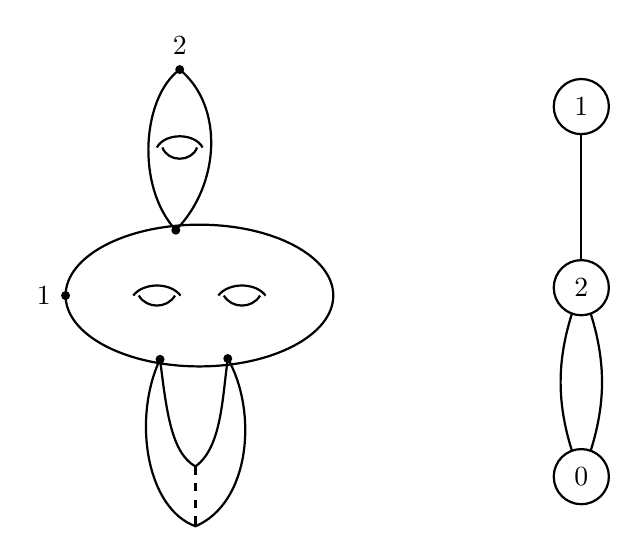
\begin{tikzpicture}[
        x=1cm,
        y=1cm,
        curve component/.style={thick},
        marked point/.style={circle,fill=black,inner sep=1.15pt},
        graph vertex/.style={
            circle,draw,thick,fill=white,minimum size=7mm,inner sep=0pt
        }
    ]
        % A three-component curve with components of genera 1, 2, and 0.
        \draw[curve component] (1.5,3.65) ellipse [x radius=1.7,y radius=0.9];

        % The two handles on the genus-two component.
        \draw[curve component]
            (0.66,3.65)
            .. controls (0.79,3.82) and (1.13,3.82) .. (1.26,3.65);
        \draw[curve component]
            (0.73,3.65)
            .. controls (0.83,3.48) and (1.09,3.48) .. (1.19,3.65);
        \draw[curve component]
            (1.74,3.65)
            .. controls (1.87,3.82) and (2.21,3.82) .. (2.34,3.65);
        \draw[curve component]
            (1.81,3.65)
            .. controls (1.91,3.48) and (2.17,3.48) .. (2.27,3.65);

        % The genus-one component attached above.
        \coordinate (uppernode) at (1.2,4.48);
        \draw[curve component]
            (uppernode)
            .. controls (0.68,5.05) and (0.78,6.18) .. (1.25,6.52)
            .. controls (1.82,6.05) and (1.76,5.05) .. cycle;
        \draw[curve component]
            (0.96,5.53)
            .. controls (1.06,5.72) and (1.44,5.72) .. (1.54,5.53);
        \draw[curve component]
            (1.03,5.53)
            .. controls (1.10,5.34) and (1.40,5.34) .. (1.47,5.53);

        % The rational component attached at two nodes below.
        \coordinate (lowerleft) at (1.00,2.84);
        \coordinate (lowerright) at (1.86,2.85);
        \draw[curve component]
            (lowerleft)
            .. controls (0.65,2.10) and (0.82,0.95) .. (1.45,0.72)
            .. controls (2.15,1.02) and (2.24,2.18) .. (lowerright);
        \draw[curve component]
            (lowerleft)
            .. controls (1.08,2.20) and (1.14,1.65) .. (1.45,1.48)
            .. controls (1.78,1.72) and (1.79,2.34) .. (lowerright);
        \draw[curve component,dashed] (1.45,1.48) -- (1.45,0.72);

        % Nodes and marked points.
        \node[marked point] at (uppernode) {};
        \node[marked point] at (lowerleft) {};
        \node[marked point] at (lowerright) {};
        \node[marked point,label=left:{$1$}] at (-0.2,3.65) {};
        \node[marked point,label=above:{$2$}] at (1.25,6.52) {};

        % The dual graph: the vertex labels record the genera.
        \coordinate (vone) at (6.35,6.05);
        \coordinate (vtwo) at (6.35,3.75);
        \coordinate (vzero) at (6.35,1.35);
        \draw[curve component] (vone) -- (vtwo);
        \draw[curve component]
            (vtwo) to[out=-112,in=112] (vzero);
        \draw[curve component]
            (vtwo) to[out=-68,in=68] (vzero);
        \node[graph vertex] at (vone) {$1$};
        \node[graph vertex] at (vtwo) {$2$};
        \node[graph vertex] at (vzero) {$0$};
    \end{tikzpicture}
    \end{center}
\end{exm}

对于一个对数或穿孔 R-映射
\begin{equation*}
\begin{tikzcd}
    & \mf{P} \ar{d} \\
    C \ar{ur}{f} \ar{d} \ar{r} & B \C_{\omega}^{\times} \\
    S,
\end{tikzcd}
\end{equation*}
我们通过取整个图的相伴广义锥复形来将其热带化。因为 \(B \C_{\omega}^{\times}\) 没有对数结构，我们看到的是
\begin{equation*}
\begin{tikzcd}
    \Sigma(C) \ar{d} \ar{r}{\Sigma(f)} & \Sigma(\mf{P}) = \R_{\geq 0} \\
    \Sigma(S).
\end{tikzcd}
\end{equation*}
现在设 \(S = \Spec (Q \to \C)\) 是一个对数点，其中 \(Q\) 是一个 fs 尖锐幺半群。特别地，这意味着 \(\Sigma(S) = Q_{\R}^{\vee}\)。因为一切都是（分段）线性的，只需考虑一个内点 \(t \in \Sigma(S)\) 并考察 \(\Sigma(C)_t\)。

我们把每条半边视为从其所附着的顶点指向外部；特别地，这意味着一个到 \(\R_{\geq 0}\) 的线性映射对应于一个斜率。我们称之为\textit{接触阶}。特别地，若 \(h \neq \hat{h}\) 由 \(\imath\) 相关联，则有 \(c(h) = - c(\hat{h})\)。对所有 \(v \in \V\)，我们还定义\textit{退化度}
\[ e_v \colon Q_{\R}^{\vee} \to \R_{\geq 0} \qquad t \mapsto \Sigma(f)_t (v). \]
特别地，\(e_v \in Q\) 是一个整点。

接下来需要介绍的是穿孔腿。它们记为
\[ \L^{\circ} = \ab\{ h \in \H \mid \Sigma(f)_t(h) \text{ is bounded and nontrivial for all } t \in Q_{\R}^{\vee}\}. \] 
我们定义在 \(h \in \L^{\circ}\) 处的预稳定性为 \(0 \in \ol{\Sigma(f)_t(h)}\)，这是一个技术上必要的假设。在所有穿孔腿都预稳定的假设下，我们可以定义\textit{边长}函数
\[ \ell \colon \E \cup \L^{\circ} \to \ms{Map}(Q_{\R}^{\vee}, \R_{\geq 0}) \qquad x \mapsto \ell(x) \colon t \mapsto \ell(x)(t). \]
注意到对于边 \(E\)，\(\ell(E) \in Q\) 也是整点。对于穿孔腿，这在相差细分的意义下成立。

\subsection{对数 GLSM 不变量}%
\label{sub:Log GLSM invariants}

\begin{defn}
    我们定义对数映射 \(f\) 的\textit{带装饰的热带型}为
    \[ \bm{\tau} = (G, c \colon \H \to \Z, \beta \colon \V \to H_2(X)). \]
\end{defn}

\begin{defn}
    一个对数或穿孔映射 \(f\) 称为\textit{紧型}的，如果
    \begin{enumerate}
        \item 对所有 \(t\)，\(\Ima \Sigma(f)_t\) 有界；
        \item 对所有接触阶为 \(0\) 的半边 \(h\)，有 \(f(p_h) \in 0_{\mf{P}}\)。
    \end{enumerate}
\end{defn}

现在我们可以定义稳定穿孔 R-映射的范畴 \(\mc{R}(\mf{P}, \tau)\)，它纤维于 fs 对数概形的范畴 \(\ms{LogSch}\) 之上，并由 \(\tau\) 标记。

\begin{thm}[{\cite{CJR2021,CJRpunctured}}]
    栈 \(\mc{R}(\mf{P},\bm{\tau})\) 由一个带有基本/极小对数结构的本征 DM 栈表示。
\end{thm}

\begin{rmk}
    若 \(\V = \ab\{v\}\) 是独点集，则我们记
    \[ \mc{R}_{g, c}(\mf{P}, \beta) \coloneqq \mc{R}(\mf{P}, \bm{\tau}). \]
\end{rmk}

考虑图
\begin{equation*}
\begin{tikzcd}
    & \mf{P} \ar{d} \\
    \mc{C} \ar{ur}{f} \ar{d}{\pi} \ar{r} & B \C_{\omega}^{\times} \\
    \mc{R},
\end{tikzcd}
\end{equation*}
其中我们令 \(\mc{R} \coloneqq \mc{R}(\mf{P}, \bm{\tau})\)。那么完美障碍理论定义为
\[ T_{\mc{R}/\ms{Log}_{\mf{M}_G}} \to \E_{\square} = R \pi_* f^* T_{\mf{P}/B\C_{\omega}^{\times}}. \]
这里，两个切丛都指对数切复形。由完美障碍理论，这定义了典范虚拟闭链
\[ [\mc{R}(\mf{P}, \bm{\tau})]^{\vir}. \]
这个虚拟闭链的主要缺点是它不能再现 Gromov--Witten 理论。然而，我们可以考察它与 GW 理论的差异，但为此我们需要一个双有理修改。设 \(Q\) 为尖锐幺半群。它带有一个偏序：\(a < b\) 当且仅当存在非零的 \(c \in Q\) 使得 \(a+c = b\)。

\begin{defn}
    我们称 \(f\) 或 \(\Sigma(f)\) 具有\textit{一致极大退化度}，如果存在 \(e_{\max} \in \ab\{e_v \mid v \in \V \}\) 使得对所有 \(v \in \V\) 都有 \(e_{\max} \geq e_v\)。
\end{defn}

\begin{rmk}
    若 \(f\) 是紧型的且具有一致极大退化度，则 \(\Sigma(f)\) 由 \(e_{\max}\) 一致有界。
\end{rmk}

\begin{defn}
    定义 \(\mc{U}(\mf{P}, \bm{\tau})\) 为由 \(\bm{\tau}\) 标记的、具有一致极大退化度的稳定穿孔或对数 R-映射的栈。
\end{defn}

\begin{rmk}
    若 \(\V = \ab\{v\}\) 是独点集，则我们记
    \[ \mc{U}_{g, c}(\mf{P}, \beta) \coloneqq \mc{U}(\mf{P}, \bm{\tau}). \]
    若接触阶中有一个为负，则我们记
    \[ \mc{U}_{g, c}(\infty, \beta) \coloneqq \mc{U}(\mf{P}, \bm{\tau}). \]
\end{rmk}

注意到顶点有两种类型：若一个顶点映到 \(0\)，则要么至少有一条半边指向上方，要么所有接触阶都为 \(0\)（此时它们全被压缩）。这些称为\textit{对数顶点}。另一种类型的顶点是不映到 \(0\) 的顶点。要么所有半边指向下方，要么存在一些指向上方的半边。这些称为\textit{\(\infty\)-顶点}。此外，紧型的顶点正是那些没有指向上方半边的顶点。

若忘掉一致极大退化度条件，则有映射
\[ \mc{U}(\mf{P}, \bm{\tau}) \xrightarrow{F} \mc{R}(\mf{P}, \bm{\tau}) \]
它是 \(\ms{LogSch}\) 上的一个子范畴。然而，作为代数栈的态射，它是对数平展、本征且满射的。此外，\(\mc{U}\) 带有一个从 \(\mc{R}\) 拉回的典范完美障碍理论。在顶点集为独点集的情形，我们有
\begin{align*}
    F_* [\mc{U}_{g, c}(\mf{P}, \beta)]^{\vir} &= [\mc{R}_{g, c}(\mf{P}, \beta)]^{\vir}; \\
    F_* [\mc{U}_{g, c}(\infty, \beta)]^{\vir} &= [\mc{R}_{g, c}(\infty, \beta)]^{\vir}.
\end{align*}
在对数顶点的情形，我们事实上有如下图所示的从带 p-场的稳定映射模空间出发的包含
\begin{equation*}
\begin{tikzcd}
    \mc{U} \ar{rr}{F} & & \mc{R} \\
    & \mc{R}_{g,c}(\mf{P}^{\circ}, \beta) \ar[hookrightarrow]{ul} \ar[hookrightarrow]{ur}.
\end{tikzcd}
\end{equation*}
若记 p-场的模空间为 \(\mc{R}^{\circ}\)，则边界
\[ \Delta \coloneqq \mc{U} \setminus \mc{R}^{\circ} \]
是一个 Cartier 除子。由一致极大退化度条件，我们有一个截面
\[ e_{\max} \in H^0(\bar{M}_{\mc{U}}). \]
这等价于一个态射
\[ \mc{U} \to ([\A^1/\G_m], 0) \]
的数据，它将 \(0\) 拉回为 \(\Delta\)。

我们定义\textit{超势}为一个函数
\begin{equation*}
\begin{tikzcd}
    \mf{P}^{\circ} \ar{rr}{W} \ar{dr} && \mc{L}_{\omega} \ar{dl} \\
    & B \C_{\omega}^{\times}.
\end{tikzcd}
\end{equation*}
其\textit{临界轨迹}记为
\[ \on{Crit}(W) = (\d{W} = 0). \]
若 \(\on{Crit}(W) \to B\C_{\omega}^{\times}\) 是本征的，我们称 \(W\) 具有\textit{本征临界轨迹}。

例如，假设我们感兴趣的是 GW 理论。设 \(X\) 为光滑射影簇，\(V\) 为 \(X\) 上的一个向量丛，\(s \in H^0(V)\)。令 \(Z = (s = 0)\)。于是我们得到
\[ W \colon \mf{P}^{\circ} = V^{\vee} \boxtimes \mc{L}_{\omega} \xrightarrow{s \otimes 1_{\omega}} \mc{L}_{\omega}. \]

\begin{lem}
    \(W\) 具有本征临界轨迹当且仅当 \(Z\) 是具有期望余维数的光滑簇。
\end{lem}

\begin{exm}
    设 \(X\) 为一个点，\(V = \C\)，且 \(s \neq 0\)。则 \(\d{W} = s \neq 0\)，故临界轨迹为空。
\end{exm}

利用 Kiem--Li 的余截面局部化方法~\cite{KiemLi2013}，我们可以得到一个虚拟闭链
\[ [\mc{R}_{g, c=n}(\mf{P}^{\circ}, \beta)]_W^{\vir}, \]
它支撑在临界轨迹上。在 GW 理论中，它等于 GW 虚拟闭链
\[ \pm [\bar{M}_{g,n}(\on{Crit}(W), \beta)]^{\vir}, \]
其中符号可以显式计算。

\begin{thm}[{\cite{CJR2021,CJW2021}}]
    设 \(\bm{\tau}\) 为紧型的。在紧型情形下，
    \begin{enumerate}
        \item \(\mc{U}(\mf{P}, \bm{\tau})\) 有一个约化完美障碍理论，它给出约化虚拟闭链 \([\mc{U}(\mf{P}, \bm{\tau})]^{\vir}\)；
        \item \(\Delta\) 有一个约化完美障碍理论，它给出约化虚拟闭链 \([\Delta]^{\vir}\)；
        \item 在单个对数顶点的情形，我们有 \([\mc{U}_{g, c=n}(\mf{P}, \beta)]^{\on{red}} = \pm [\bar{M}_{g,n}(\on{Crit}(W), \beta)]^{\vir}\)。此外，有公式
            \[ [\mc{U}_{g, c=n}(\mf{P}, \beta)]^{\on{red}} = [\mc{U}_{g, c=n}(\mf{P}, \beta)]^{\vir} - \tilde{r} [\Delta]^{\on{red}}, \]
            其中 \(\tilde{r}\) 是 \(W\) 沿 \(\infty\) 的极点阶。
    \end{enumerate}
\end{thm}

\subsection{热带分解与有限生成}%
\label{sub:Tropical decomposition and finite generation}

下述热带分解及其应用来自工作草稿~\cite{CJRtropical2025}。有效不变量及其公理在~\cite{CJRpunctured} 中建立。

从现在起，我们将考虑一个更简单的设定：\(X\) 是光滑射影簇，\(V\) 是 \(X\) 上的一个线丛。此时，我们假设 \(Z = (s = 0)\) 是余维数 \(1\) 的光滑簇。此外，我们假设 \(Z\) 是一个 Calabi--Yau 三维簇。我们将考虑不变量
\[ N_{g, \beta} \coloneqq \int_{[\bar{M}_{g,0}(Z, \beta)]^{\vir}} 1 \in \Q \]
和生成级数
\[ F_g = \sum_{\beta \geq 0} N_{g, \beta} Q^{\beta} \in \Lambda \coloneqq \C \ps{Q}. \]

\begin{conj}[Yamaguchi-Yau, Alim-L\"ange {\cite{YY2004,AlimLange2007}}]
    假设 \(g=0\) 镜面对称对 \(Z\) 成立。则存在有限生成的 \(\Q\)-代数 \(R \subset \Lambda\)，使得对所有 \(g \geq 2\)，有 \(F_g \in (I_0(q))^{2g-2} R\)。
\end{conj}

我们的主要目标如下。

\begin{thm}[{\cite{CJRtropical2025}}]
    设 \(Z\) 是没有奇次上同调的 Fano 四维簇 \(X\) 中的一个 Calabi--Yau 三维超曲面。设 \(\{\phi_j\}\) 为 \(H^*(X)\) 的一组基，\(\ab\{\phi^j\}\) 为其对偶基。则对所有 \(g \geq 0\)，我们有
    \begin{align*}
        &F_g = (-1)^{1-g} \sum_{\tau' \in G_g'} \frac{(-1)^{\abs{\V_{\infty}}}}{\abs{\Aut(\tau')}} \cdot \prod_{E \in \E} c(E) \\
        & \cdot \sum_{j_E \mid E = \ab\{E_{\log}, E_{\infty}\} \in \E} \prod_{\substack{v \in \V_{\infty} \\ g(v)=1 \\ \H_v = \ab\{E_{\infty}\}}} c_1^{\mr{eff}}(\phi^{j_E}) \cdot \prod_{\substack{v \in \V_{\infty} \\ g(v) \geq 2}} \tilde{Q}^{\beta(v)} \cdot \exp \ab(\int_{\beta(v)} K(Q) )  \\
        & \cdot \ab(\prod_{E_{\infty} \in \H_v'}\int_{\beta(v)} \phi^{j_E}) \cdot c_{g(v), \beta(v)}^{\on{eff}} 
         \cdot \prod_{v \in \V_{\log}} \Omega_{g(v), \abs{\H_1(v)}, \abs{\H_2(v)}} (\phi_{j_E} \colon E_{\log} \in \H_1(v)).
    \end{align*}
\end{thm}

\begin{exm}
    设 \(Y\) 为带有其环对数结构的环簇。则 \(\Sigma(Y)\) 是视为锥复形的环扇，我们可以考虑其边界 \(\Delta_Y = \sum_{\rho \in \Sigma(Y)^1} \Delta_{\rho}\)。 
\end{exm}

若考虑 \([\Delta]^{\on{red}}\)，我们应当得到类似的公式
\[ [\Delta]^{\on{red}} = \sum_{\rho \in \Sigma(\Delta)(1)} [\Delta_{\rho}]^{\on{red}}. \]
现在的问题是这些 \(\rho\) 代表什么。事实上，它们参数化了刚性热带曲线。在热带化
\begin{equation*}
\begin{tikzcd}
    \Sigma(C)_{\rho} \ar{d} \ar{r} & \Sigma(\mc{C}) \ar{r}{f} \ar{d} & \R_{\geq 0} \\
    \rho \ar[hookrightarrow]{r} & \Sigma(\mc{U}),
\end{tikzcd}
\end{equation*}
中，我们看到 \(f_{\rho}\) 是刚性的当且仅当源热带曲线是一个二部图，其一组顶点映到 \(e_{\max}\)，另一组顶点映到 \(0\)。

\begin{exm}
    设 \(X\) 为一个点，\(Z = \emptyset\)。再考虑 \(g = 2, n = 0\)。此时可能的图由~\Cref{fig:tropgraphs} 给出。
    \begin{figure}[htpb]
    \begin{center}
    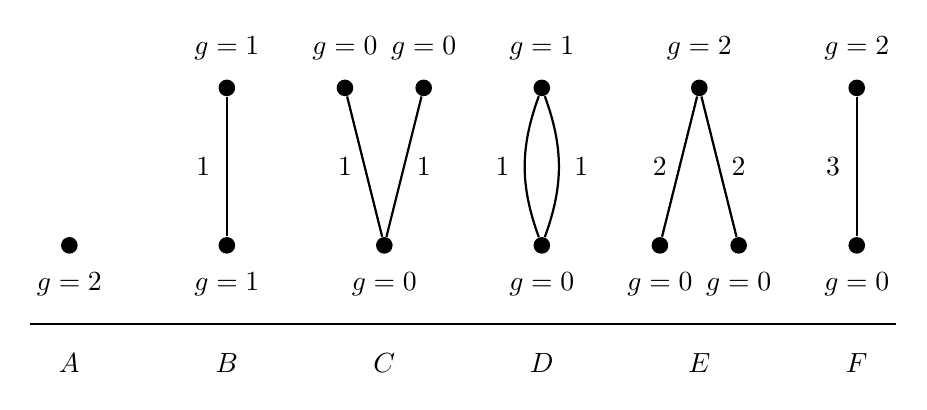
\begin{tikzpicture}[scale=1, transform shape]
        \node[fill=black,circle,minimum size=6pt,inner sep=0pt] (A) at (0,0) {};
        \node[fill=black,circle,minimum size=6pt,inner sep=0pt] (B1) at (2,0) {};
        \node[fill=black,circle,minimum size=6pt,inner sep=0pt] (B2) at (2,2) {};
        \node[fill=black,circle,minimum size=6pt,inner sep=0pt] (C1) at (4,0) {};
        \node[fill=black,circle,minimum size=6pt,inner sep=0pt] (C2) at (3.5,2) {};
        \node[fill=black,circle,minimum size=6pt,inner sep=0pt] (C3) at (4.5,2) {};
        \node[fill=black,circle,minimum size=6pt,inner sep=0pt] (D1) at (6,0) {};
        \node[fill=black,circle,minimum size=6pt,inner sep=0pt] (D2) at (6,2) {};
        \node[fill=black,circle,minimum size=6pt,inner sep=0pt] (E1) at (8,2) {};
        \node[fill=black,circle,minimum size=6pt,inner sep=0pt] (E2) at (7.5,0) {};
        \node[fill=black,circle,minimum size=6pt,inner sep=0pt] (E3) at (8.5,0) {};
        \node[fill=black,circle,minimum size=6pt,inner sep=0pt] (F1) at (10,0) {};
        \node[fill=black,circle,minimum size=6pt,inner sep=0pt] (F2) at (10,2) {};
        \draw[-,thick] (B1) -- (B2);
        \draw[-,thick] (C2) -- (C1) -- (C3);
        \draw[-,thick] (D1) edge[bend left=20] (D2);
        \draw[-,thick] (D2) edge[bend left=20] (D1);
        \draw[-,thick] (E2) -- (E1) -- (E3);
        \draw[-,thick] (F1) -- (F2);
        \node at (0,-0.5) {$g=2$};
        \node at (2,-0.5) {$g=1$};
        \node at (4,-0.5) {$g=0$};
        \node at (6,-0.5) {$g=0$};
        \node at (7.5,-0.5) {$g=0$};
        \node at (8.5,-0.5) {$g=0$};
        \node at (10,-0.5) {$g=0$};
        \node at (2,2.5) {$g=1$};
        \node at (3.5,2.5) {$g=0$};
        \node at (4.5,2.5) {$g=0$};
        \node at (6,2.5) {$g=1$};
        \node at (8,2.5) {$g=2$};
        \node at (10,2.5) {$g=2$};
        \draw[-,thick] (-0.5,-1) -- (10.5,-1);
        \node at (0,-1.5) {$A$};
        \node at (2,-1.5) {$B$};
        \node at (4,-1.5) {$C$};
        \node at (6,-1.5) {$D$};
        \node at (8,-1.5) {$E$};
        \node at (10,-1.5) {$F$};
        \node at (1.7,1) {$1$};
        \node at (3.5,1) {$1$};
        \node at (4.5,1) {$1$};
        \node at (5.5,1) {$1$};
        \node at (6.5,1) {$1$};
        \node at (7.5,1) {$2$};
        \node at (8.5,1) {$2$};
        \node at (9.7,1) {$3$};
    \end{tikzpicture}
    \end{center}
        \caption{当 $g=2$ 时，$X = \mr{pt}$ 且 \(Z = \emptyset\) 情形的热带型的图。}%
    \label{fig:tropgraphs}
    \end{figure}
\end{exm}

\begin{thm}[热带量子 Lefschetz {\cite{CJRtropical2025}}]
    设 \(X\) 与 \(Z\) 如前。对任意 \(\beta \in H_2(X)\)、任意 \(\alpha_1, \ldots, \alpha_n \in H^*(X)\) 以及任意 \(k_1, \ldots, k_n \in \N\)，我们有
    \begin{align*}
        \int_{[\bar{M}_{g,n}(Z,\beta)]^{\vir}} \prod_{j=1}^n \ev_j^* (\alpha_j) \psi^{k_j}={}& (-1)^{1-g+\beta \cdot Z} \cdot \sum_{\tau \vdash (g,n,\beta)} \frac{(-1)^{\abs{\V_{\infty}}}}{\abs{\Aut(\tau)}} \cdot \prod_{E \in \E} c(E) \\
        & \cdot \sum_{\ab\{j_E \mid E = \ab\{E_{\log}, E_{\infty}\}\}}  \prod_{v \in \V_{\infty}} \int_{[\mc{U}_v]^{\on{red}}} \prod_{E_{\infty} \in \H_v} \ev_{E_{\infty}}^* \phi^{j_E}  \\
        &  \cdot \prod_{v \in \V_{\log}} \int_{[\mc{R}_v]^{\vir}} \prod_{E_{\log}} \ev_{E_{\log}}^* (\phi_{j_E}) \cdot \prod_{h \in \L_v} \ev_h^* \alpha_h \cdot \psi_h^{k_h} .
    \end{align*}
\end{thm}

\begin{rmk}
    还有一个虚拟局部化公式，已在~\cite{CJRlocalization} 中宣布，它既可用于约化理论（仅有 R-环面作用），也可用于典范理论（可用于外围空间的全部自同构）。
\end{rmk}

现在考虑一个 \(\infty\)-顶点。令 \(\tau_v = (g, c, \beta)\)，并令 \(\mc{U}_v = \mc{U}_{g,c}(\infty, \beta)\)。那么第一个计算是
\begin{align*}
    \on{red}\dim \mc{U}_v &= \chi(f^* T_{\mf{P}/B \C^{\times}_{\omega}}) + 1 + \on{trop}\dim  \\
    &= \vir\dim \bar{M}_{g,n}(Z, \beta) + \sum_{h \in \H } (c(h) + 1),
\end{align*}
其中热带维数为 \(3g-4+n\)。注意到所有接触阶都是负的，所以第二项至多为零。特别地，我们证明了
\begin{cor}[{\cite{CJRpunctured}}]
    若 \(\vir\dim \bar{M}_{g,n}(Z,\beta) < 0\)，则 \([\mc{U}_v]^{\on{red}} = 0\)。
\end{cor}
我们还有\textit{平衡条件}，即
\begin{equation}\label{eqn:balancing condition}
    \sum_{h \in \H} c(h) = \deg f^* \mc{O}(\infty) = \int_{\beta} c_1(V) - (2g-2+n).
\end{equation}
它可以改写为
\[ 0 \geq \sum_{h \in \H} (c(h)+1) = \int_{\beta} c_1(V) - (2g-2). \]
\begin{prop}[{\cite{CJRpunctured}}]
    我们看到在下列情形下不存在 \(\infty\)-顶点：
    \begin{enumerate}
        \item \(g = 0\) 且 \(V\) 是 nef 的；
        \item \(g=1\) 且 \(V\) 是丰沛的，除非 \(\beta = 0\) 且所有 \(c(h) = -1\)。
    \end{enumerate}
\end{prop}

\begin{defn}
    一个标记称为\textit{单位}，如果其接触阶为 \(-1\)。
\end{defn}

\begin{notn}
    我们将单位扇形记为 \(\1\)，并记 \(\tau_{v+\1} = (g, c+\1, \beta)\)、\(\mc{U}_{v+\1} = \mc{U}_{g, c+\1}(\infty, \beta)\) 和 \(\mc{R}_{v+\1} = \mc{R}_{g, c+\1}(\infty, \beta)\)。
\end{notn}

\begin{thm}[{\cite[Theorems~1.16--1.17]{CJRpunctured}}]\leavevmode
    \begin{enumerate}
        \item 存在映射 \(F_{\1} \colon \mc{U}_{v+\1} \xrightarrow{s} \mc{C}^{\circ} \xrightarrow{\pi} \mc{U}_v\)，其中 \(s\) 是双有理的；
        \item 我们有约化虚拟闭链的等式 \(s_* [\mc{U}_{v+\1}]^{\on{red}} = \pi^* [\mc{U}_v]^{\on{red}}\)；
        \item 若 \(D\) 是 \(X\) 上的一个除子，则 \(F_{\1 *} (\ev_{\1}^* D \cap [\mc{U}_{v+\1}]^{\on{red}}) = \ab(\int_{\beta} D) [\mc{U}_v]^{\on{red}}\)； 
        \item 考虑图
            \begin{equation*}
            \begin{tikzcd}
                \mc{U}_{v+\1} \ar{r}{F} \ar{d}[swap]{F_{\1}} & \bar{M}_{g,n+1} \ar{d}[swap]{p} \\
                \mc{U}_v \ar{r}{F} & \bar{M}_{g,n}.
            \end{tikzcd}
            \end{equation*}
            则 \(F_* [\mc{U}_{v+\1}]^{\on{red}} = p^* F_* [\mc{U}_v]^{\on{red}}\)。
    \end{enumerate}
\end{thm}

\begin{exm}
    考虑如下设定：\(g = 1\) 且 \(Z_d \subset X = \P^N\) 是一个超曲面。我们只需考虑 \(\beta = 0\) 且对所有 \(h \in \H\) 有 \(c(h) = -1\) 的情形。于是我们看到
    \[ \prod_h \ev_h^* \alpha_h \cdot [\mc{U}_{1,c}(\infty,\beta)]^{\mr{red}} = \ev_{h^{\star}}^* \ab(\prod_h \alpha_h) \cap [\mc{U}_{1,\1}(\infty,\beta)]^{\on{red}}. \]
\end{exm}

\begin{prop}[{\cite{CJRpunctured}}]
    我们事实上有
    \[ \mc{U}_{1,\1}(\infty, 0) \simeq \mc{R}_{1,\1}(\infty, 0) \]
    以及等式
    \[ [\mc{U}_{1,\1}(\infty, 0)]^{\on{red}} = c_{\dim X} \ab(\mc{H}^{\vee} \boxtimes T_{\mf{P}/B\C_{\omega}^{\times}} + \mc{O} - V). \]
\end{prop}

\begin{exm}
    现在考虑五次三维簇 \(Z_5 \subset \P^4\)。于是我们看到 \(\on{red}\dim \mc{U}_v = \sum_{h \in \H} (c(h)+2)\)。单位公理把我们归结到 \(c(h) \leq -2\) 的情形。现在我们必须确定当所有 \(c(h) = -2\) 时需要考虑的新不变量的个数，这等价于找出可能的 \(\beta\) 的个数。平衡条件给出
    \begin{align*}
        \sum_{h \in \H} c(h) &= \int_{\beta} c_1(V) - (2g-2+n) \\
        &= 5\beta - (2g-2+n),
    \end{align*}
    这意味着 \(0 \geq \sum (c(h)+1) = 5\beta - (2g-2)\)，从而 \(\beta \leq \frac{2g-2}{5}\)。\footnote{若假设有限生成、全纯反常方程、轨形正则性和锥形点间隙条件，这正好就是所预言的未知量的个数。}
\end{exm}

\begin{conj}[Janda {\cite[Conjecture~1.6]{CJRtropical2025}}]\leavevmode
    \begin{enumerate}
        \item 我们有 \(K(Q) = \log I_0(q) \cdot c_1(K_X^{\vee}) - \frac{I_1}{I_0}\) \\
        \item 典范理论满足 \(\Omega \in I_0(q)^{2g-2+2n_1 + 3 n_2} \cdot R\)。 
    \end{enumerate}
\end{conj}

\begin{cor}[{\cite[Theorem~1.7]{CJRtropical2025}}]
    上述关于 \((X, V)\) 的猜想蕴含 \(Z\) 的 Yamaguchi-Yau 有限生成。
\end{cor}

